% Tipus de document
\documentclass[a4paper]{report}
% Utilitzar tota l'amplada de la pàgina
\usepackage{fullpage}
% Extres de LaTex
\usepackage{latexsym}
% Text en utf8
\usepackage{ucs}
\usepackage[utf8x]{inputenc}
% Text generat automàticament en català i partició per síl·labes
\usepackage[catalan]{babel}
% Per afegir imatges
\usepackage{graphicx}
% Per utilitzar colors
\usepackage[usenames,dvipsnames]{color}
\usepackage[table]{xcolor}
% Pel glossari
\usepackage{nomencl} 
\makenomenclature

% Per afegir codi font
\usepackage{fancyvrb}
% Per el simbol d'euro
\usepackage{eurosym}

\include{pygmentize}
% Que mostri la capçalera a tots els fulls
%\pagestyle{headings}
\usepackage{longtable} 
% Incloure pàgines amb format pdf
\usepackage{pdfpages}


% Interliniat de 1.5
\renewcommand{\baselinestretch}{1.5}

% Autor
\author{Albert Sellarès Torra \texttt{<whats@wekk.net>}\\
		Facultat d'Informàtica de Barcelona,\\
		UPC\\}
%\date{2009}
		
% Títol de l'article
\title{skd: Rootkit per sistemes operatius UNIX}

% Millora el pdf. Ha de ser l'últim del preàmbul
\usepackage[pdftex,bookmarks,colorlinks,pdfnewwindow]{hyperref}
% Descomentar-ho per imprimir sense colors
\hypersetup{
	hyperindex=true,
	colorlinks=true,
	linkcolor=blue,
	anchorcolor=blue,
	citecolor=blue,
	filecolor=blue, 
	menucolor=blue,
	pagecolor=blue,
	urlcolor=blue,
	bookmarksnumbered=true}

\begin{document}

\large
% Portada
\includepdf[pages=-]{Portada.pdf}
%\maketitle
\newpage


% Índex
\include{index}

% Introducció

\PrerenderUnicode{ó}
\chapter{Introducció}

Aquest projecte tracta d'implementar una prova de concepte del què seria un rootkit\footnote{rootkit:
Eina o conjunt d'eines que té com a finalitat amagar-se a i amagar altres programes, processos, arxius, 
directoris, ports, etc., per tal que permeti a un intrús accedir al sistema (normalment remotament), 
així com extreure informació.} per a sistemes operatius actuals basats en UNIX.\\ 

Un rootkit és una aplicació pensada per a ser utilitzada com a porta del darrere per tal de
poder accedir i controlar un sistema, i que a més, s'amaga per a no ser descobert.\\

És sabut que existeixen programes fets amb aquesta finalitat, però la majoria d'ells són
per sistemes Windows, no estan públics a la xarxa, estan desfasats i ja no poden ser
usats en els sistemes operatius actuals. A més, els nuclis de sistemes operatius actuals implementen cada vegada més
proteccions per tal d'evitar que programes com aquests els controlin.

\section{Motivació del projecte}

Avui en dia ens veiem immersos en la societat de la informació, un moment en què la
majoria de les empreses i persones intentem adaptar-nos a les noves tecnologies,
moment en què s'intenta digitalitzar tot el què es pot. Qui més qui menys veu que en uns anys tot es veurà gestionat a través de sistemes
d'informació, tot estarà interconnectat entre sí, i s'ha de poder garantir que tots aquests
sistemes comptin amb un mínim de seguretat.\\


Les implicacions que té estar infectat per un virus estan canviant. Els virus (i en particular
els cavalls de Troia) ja no es fan per molestar a l'usuari, al contrari, un alt percentatge dels
virus tenen com a objectiu principal ocultar-se. Passant desapercebuts, permeten a l'infectant
controlar la nostre màquina podent fer qualsevol cosa en ella com per exemple, apoderar-
se de la nostra compta bancària.\\
Parem-nos a pensar per un moment què passaria si en comptes de què l'infecció estigués
a la nostre màquina, aquesta estigués als servidors on es fan les nostres nòmines, als dels
nostres bancs, o a les de qualsevol pàgina de venta d'articles per internet. El perill i la
criticitat es disparen exponencialment.\\


Des dels inicis de la història els sistemes operatius UNIX han estat al capdavant en els
entorns de servidors, i des de llavors que les grans empreses els utilitzen per a confiar-hi
les seves dades. Avui, i gràcies al boom que ha fet el GNU/Linux i en general el programari lliure (tothom qui més qui
menys té una idea del què és), administradors de sistemes no experimentats acaben
utilitzant sistemes basats en UNIX en el seu lloc de treball. \\
El fet és, que actualment moltes empreses utilitzen aquests sistemes operatius (com poden ser
GNU/Linux, BSD, Solaris, etc) per als seus servidors, i són moltes les què s'acaben despreocupant
de la seguretat dels servidors donant com a excusa que un sistema basat amb UNIX és
més segur, i que a més, no hi han virus. A la practica, molta gent que es dedica a
administrar aquestes màquines, no està qualificada, o no compta amb el temps necessari
per a fer-ho del tot bé, i com que les coses aparentment funcionen, es segueix així. \\

I aquest és el punt on vull arribar. Avui, una persona amb suficients ganes, temps i
coneixements, pot guanyar accés a la majoria de servidors, on un cop dintre, la seva
preocupació principal és mantenir-ne l'accés.\\

Amb aquest projecte intento posar de manifest, creant una prova del concepte, lo difícil
que pot arribar a ser per un administrador de sistemes adonar-se que ha estat infectat per
un rootkit, lo perillós per a la seguretat del sistema, i lo crua que és la realitat ja que un
intrús pot tenir-ho molt fàcil per a controlar el nostre servidor.

\section{Objectiu}

L'objectiu del projecte és implementar un rootkit per a sistemes basats en UNIX. Tot seguit
es descriu en forma de resum, les característiques en un caire general que el rootkit ha de potenciar. 

\begin{description}
    \item[Ocultació] Ha de passar el màxim desapercebut en el sistema on estigui
    instal·lat. Per un administrador, ha de ser molt difícil adonar-se que el
    sistema ha estat compromès. El rootkit ha d'intentar ocultar al màxim les tasques
    que executa.

    \item[Accés] Ha de permetre l'accés a la persona que
    l'ha instal·lat. Normalment i per comoditat, aquest accés és remot a través
    d'internet. El rootkit ha de facilitar al màxim aquest accés, havent d'evitar les diferents 
    barreres que hi puguin haver (firewalls, ACLs, etc).

    \item[Administració] Ha de permetre realitzar tot tipus
    d'accions a la màquina com si d'un usuari vàlid es tractés. Accions com executar
    tasques, editar fitxers, pujar o descarregar-ne, són funcionalitats bàsiques que ens
    ha de permetre efectuar.

    \item[Permanència] Les màquines s'actualitzen, es paren i s'engeguen. El rootkit ha
    d'intentar no veure's afectat per aquests canvis.

    \item[Augment de privilegis] Ha d'ajudar tant com pugui, a l'obtenció de nous
    privilegis. Altres comptes d'usuari, comptes d'altres màquines, comptes de bases de dades, etc.
\end{description}



% Definició del problema o requeriments
\chapter{Definició del problema}

Per tal de poder entendre la necessitat de les diferents funcionalitats que ens ha d'oferir el rootkit,
és important que primer de tot, tinguem una idea de com es realitzen avui en dia la gran majoria
d'intrusions\footnote{Una intrusió, és l'accés il·legal a una màquina. El fet de introduir-se a una màquina
en temes de seguretat informàtica, també s'acostuma a dir (en un llenguatge més informal) ``hackejar una màquina''},
i el què fan els diferents administradors per protegir-se. Cal tenir en compte que aquests procediments són 
utilitzats alhora d'atacar servidors, en cas de voler atacar pc's d'usuaris domèstics, les tècniques utilitzades 
solen ser diferents.

\section{Intrusions}

Una intrusió és el fet d'aconseguir accés a una màquina normalment remota. D'una manera més tècnica, es podria dir
que l'objectiu d'una intrusió és poder arribar a executar codi\footnote{Amb codi ens referim a llenguatge màquina o comandes de sistema.} 
a la màquina víctima. \\

La intrusió és el primer pas necessari per tal de poder comprometre del tot una màquina. El conjunt de passos a 
realitzar alhora d'accedir a una màquina es poden resumir com:

\begin{itemize}
\item Intrusió.
\item Augment de privilegis.
\item Instal·lació d'un backdoor.
\item Eliminació de proves.
\end{itemize}

Aquests són els passos a realitzar en una ``bona'' intrusió, tot i que a la majoria de les intrusions que es produeixen
avui en dia són processos automatitzats que només realitzen el primer i tercer punt.

\subsection{Intrusions automatitzades} 

Avui en dia, la majoria d'intrusions que pateixen els servidors, són intrusions automatitzades causades per cucs o 
programes que exploten un bug o mala configuració en un software en concret. Aquestes intrusions automatitzen les 
tasques a executar un cop s'aconsegueix l'accés a una màquina, així com el mateix procediment per aconseguir accedir-hi. 
Per tal de trobar possibles víctimes, aquests programes
es dediquen a escanejar diferents rangs d'IPs a la cerca de màquines que tinguin un servei en qüestió, o 
fan de crawler per tal de trobar noves URLs que indiquin l'ús d'un software web vulnerable. \\

A una màquina víctima d'una intrusió com aquesta, se li instal·la un tipus de rootkit que permet llançar accions en 
ella (un backdoor). Fins fa poc, la majoria de backdoors d'aquest tipus es connectaven a canals de IRC, on 
processaven les comandes que algun altre usuari llançava. D'aquesta manera, el propietari del backdoor podia controlar 
d'una manera fàcil moltes màquines alhora. Per tal de llançar alguna acció en les víctimes, aquest usuari només havia de 
connectar-se al canal en qüestió, i 
enviar un missatge de text, que seria interpretat per totes les màquines que tinguessin el seu backdoor instal·lat. 
Recentment tot això ha començat a canviar una mica, ja que els propietaris d'aquests backdoors estan millorant força la tècnica
per fer-los més efectius. \\

El conjunt de màquines infectades per aquest tipus de backdoors, i que poden ser controlades totes alhora, s'anomena
botnets. Aquestes botnets s'utilitzen principalment per fer atacs massius de tipus DoS contra altres màquines i per enviar SPAM. 
Una dada interessant, és el fet que hi ha gent que s'hi guanya la vida. Per exemple, per una xarxa d'unes 10.000 màquines
es poden arribar a pagar quantitats entre 15.000 USD i 20.000 USD. \\

El principal canvi que estan realitzant la majoria d'aquests backdoors, és que estan canviant el protocol de funcionament. Els
més moderns que han aparegut, han canviat l'IRC per l'HTTP i a més, han implementant tècniques de xifratge sobre els diferents 
missatges amb l'objectiu de passar més desapercebuts\footnote{Un exemple d'això, és la recent notícia de que el servei web 
\href{http://twitter.com/}{Twitter} estava sent utilitzat per a controlar una botnet \url{http://asert.arbornetworks.com/2009/08/twitter-based-botnet-command-channel/}}. \\

Les intrusions d'aquest tipus, acostumen a ser provocades per persones que realment no tenen molts coneixements tècnics, sinó que 
agafen algun exploit que s'hagi publicat recentment, i l'intenten modificar per tal de poder fer-ne un atac massiu. El
software utilitzat per gestionar la màquina, no està fet per ells sinó que el descarreguen d'Internet i el configuren. 
Aquestes intrusions acostumen a ser portades a terme per gent força jove. \\

Evitar una intrusió d'aquest tipus, acostuma a ser fàcil, ja que 
acostuma a ser suficient en mantenir tot el software de les màquines actualitzat. \\

Generalment, detectar aquest tipus d'intrusions no és molt difícil. Per detectar-les, sol ser suficient en buscar en el directori /tmp i /var/tmp
l'existència de fitxers o directoris estranys (ocults, amb espais, etc). També acostuma a ser interessant comprovar 
les connexions de xarxa per detectar si la màquina està registrada en alguna botnet. \\

\subsection{Intrusions manuals}

Les intrusions manuals depenen molt més de la persona que hi ha darrere la intrusió. \\

La menys perillosa és aquella que és realitzada per un script kiddie o newbie (el què pretén ser un hacker novell) que 
el què farà, serà semblant al propietari de la botnet, però de forma manual. Si la intrusió és satisfactòria, probablement
l'atacant intentarà augmentar els seus privilegis, i deixar algun backdoor per tal de poder mantenir l'accés que ha aconseguit
sense haver de tornar a explotar la vulnerabilitat. Cal tenir en compte que aquestes intrusions acostumen a formar part
de l'aprenentatge de la persona. \\

La intrusió realment perillosa és la que pot realitzar una persona amb una base tècnica important. En aquest cas, utilitzar
versions de software en les que no ha estat publicada cap vulnerabilitat, no és suficient (poden haver-hi vulnerabilitats
no conegudes públicament). En aquestes intrusions, l'objectiu sol estar més clar que en els anteriors (ja que 
l'esforç per realitzar-les és molt superior) i pot anar dirigit tant a aplicacions comunes, com a aplicacions fetes a mida. \\

En aquestes intrusions, i depenent de l'objectiu de l'atacant, molt probablement es realitzaran tots els punts comentats anteriorment
per tal de mantenir l'accés i passar desapercebut.  \\

En les intrusions manuals, l'atacant intentarà en tot moment treballar al màxim de còmode.
Això vol dir que si és capaç d'executar shellcode a la màquina que està atacant, no es dedicarà a crear el shellcode
necessari per a cada comanda que vulgui executar al sistema, sinó que tant aviat com pugui cercarà com
aconseguir una shell remota. Aquesta li permetrà d'una manera més o menys còmode, moure's pel sistema i llançar comandes una 
darrere l'altre. \\

Molt probablement en aquesta intrusió, un cop l'atacant hagi acabat, intentarà borrar les dades que demostren que
ha aconseguit l'accés (ex: línies de log del servei que ha explotat).

\section{Mesures de protecció}

Les principals mesures de protecció que es porten a terme per part dels administradors de sistema, per tal d'evitar
intrusions, són les següents:

\begin{description}
    \item[Actualitzacions de seguretat] La principal mesura que ajuda a mantenir els sistemes segurs, és
        realitzar les actualitzacions de seguretat, ja que aquestes corregeixen totes les vulnerabilitats
        conegudes del software instal·lat a través dels gestors de paquets del sistema operatiu. Cal tenir 
        en compte, que totes les aplicacions externes instal·lades manualment, requereixen d'una actualització i 
        comprovació manual. El fet d'instal·lar software d'aquesta manera acostuma a portar forces problemes 
        a la llarga, ja que si l'administrador no està molt al corrent del programari que instal·la,
        quan apareixen vulnerabilitats, li passen desapercebudes i a la màquina hi acaba quedant un software 
        vulnerable i mig oblidat.
    \item[Firewall d'entrada] La segona mesura que s'acostuma a aplicar a la vida real, és el fet de configurar
        un firewall que només permeti accedir als serveis que realment s'estan oferint a la màquina, de manera
        que si algun servei que està instal·lat a la màquina no ha de ser accessible des de fora, el firewall
        no hi permet l'accés. Això evita en el cas d'una intrusió, el poder deixar un servei escoltant a un port
        de la màquina de tal manera que més endavant es pugui accedir a ella.
    \item[Firewall de sortida] Un firewall de sortida ja no és una pràctica tant comuna. Només els ISPs més 
        professionals (i en definitiva, els més conscienciats amb la seguretat) són els què solen aplicar 
        polítiques de denegació del trànsit de sortida. Aplicar aquest tipus de polítiques, realment
        evita moltes possibles intrusions. Per exemple, un ISP amb aquestes polítiques però amb aplicacions 
        vulnerables instal·lades, probablement evitaria el que un possible propietari d'una botnet que utilitzés
        el IRC per controlar les màquines, s'apoderés de les seves. En aquest exemple, l'exploit explotaria 
        correctament l'aplicació vulnerable, però a l'hora de intentar connectar-se al canal de IRC per tal
        d'anunciar que està infectada, el firewall li denegaria la connexió, i així s'evitarien les 
		conseqüències de l'atac. 
        En els casos on s'utilitza un firewall de sortida, aquest no acostuma
        a denegar tot el transit, sinó que permet resolucions DNS, trànsit local, etc, i molts cops trànsit web. 
        És per aquest motiu, que les botnets estan canviant al protocol HTTP per a controlar 
        les seves màquines en comptes IRC (que era el més utilitzat fins ara).
    \item[Restriccions de sistema operatiu] A part dels punts comentats anteriorment, existeixen peces de 
        software que intenten restringir la pròpia explotació de vulnerabilitats tot endurint la seguretat que 
        envolta les aplicacions. Programari com SELinux, opcions de compilació del gcc, randomització del kernel, 
        etc, són altres tècniques que es poden utilitzar però d'una manera més involuntària ja que és 
        el propi SO el què et proveeix d'aquestes funcionalitats, i en cas de no fer-ho, és molt rara la vegada
        que una protecció d'aquestes és afegida a un sistema que no la porta ja incorporada.
    \item[Scripts personalitzats de comprovació] Una altre mesura també utilitzada, és la creació d'algun script per tal de 
        buscar processos o fitxers sospitosos. Aquesta mesura no és tant de protecció, sinó que 
        permet a l'administrador rebre una alarma en un cas concret. D'aquesta manera, és possible que 
		l'administrador pugui actuar més o menys a temps. Un script típic és el què busca execucions d'una 
		shell que pengen del procés del servidor web.
\end{description}

\section{Plans de contingència}

A part d'aquestes mesures de seguretat que permeten evitar molts incidents, els administradors de sistemes un cop
sospiten que han patit alguna intrusió, intentaran descobrir fins a on ha arribat la intrusió, què han instal·lat 
per a mantenir l'accés, i què han fet exactament. Per comprovar tot això, existeixen diferents utilitats que busquen si en 
el sistema hi han aplicacions sospitoses instal·lades. El problema que tenen aquestes utilitats és que només detecten
aplicacions genèriques, o aplicacions que utilitzen les tècniques més comunes. Exemples d'aquestes utilitats serien 
rkthunter, chckrootkit, etc. \\

En cas que aquestes utilitats no detectin res (serien com una espècie d'antivirus), poden causar a l'administrador
una falsa sensació de seguretat. Si tot i això l'administrador detecta el rootkit, ell mateix intentarà descobrir 
què és el que fa. És en aquest punt on igual  que els virus, les tècniques d'ocultació i antidebug prenen sentit.
Si l'administrador no és capaç de descobrir el què fa el rootkit, és molt possible que no el pugui eliminar de cap
altre manera que no sigui reinstal·lant la màquina. \\

\section{Objectiu}

Un cop tenim una visió més clara del què vol un atacant en el moment que realitza una intrusió, podem apropar-nos
una mica més als objectius que tindrà aquest rootkit:

\begin{itemize}
    \item Permetre recuperar l'accés i el nivell de privilegis a la màquina.
    \item Ocultar-se.
    \item Oferir un entorn el màxim de còmode.
    \item Evitar que el depurin i descobreixin el seu funcionament.
    \item Ser compatible amb la majoria de màquines.
\end{itemize}

En el nostre projecte, comencem a treballar a partir del moment en què ja hem aconseguit l'accés a la
màquina. En el moment en què ja som capaços d'executar codi, és quan volem que el nostre rootkit 
comenci a ser útil. \\


% Idea conceptual per solventar el problema
\chapter{Funcionalitats}

Un cop tenim una idea més clara del ``a què'' vol donar solució el projecte, ens cal entrar una mica més
detall en com ho vol arribar a fer. Per aquest motiu tot seguit es defineixen les diferents funcionalitats 
que ens ha d'oferir el nostre rootkit. \\

Tal i com ara veurem, les funcionalitats del rootkit, han estat separades segons els privilegis amb què s'executaria 
el rootkit.

\section{Nivells de privilegis}

En la majoria de sistemes operatius actuals, existeix una separació de privilegis entre usuaris. Hi
han diferents nivells d'usuari, tant usuaris amb molt pocs privilegis, com usuaris amb tots els privilegis
possibles. Els usuaris que disposen del màxim nivell de privilegis, s'anomenen usuaris administradors. \\
Aquests usuaris, acostumen a no tenir limitacions alhora de llançar accions a la màquina, és per aquest
motiu, que l'usuari preferit per un atacant, és l'usuari administrador. \\

\section{Entorn no privilegiat}

Aquestes són les funcionalitats que ens ofereix el rootkit quan s'executa com a \mbox{usuari no privilegiat}
\footnote{Tot i que el títol de la secció s'anomena mode no privilegiat, aquest nom no fa referència al mode d'execució
en què els nuclis dels sistemes operatius executen el codi d'usuari} del sistema.

\subsection{Executable ELF estàtic}
Per tal de fer el més portable possible el nostre rootkit, i poder així ser executat en gairebé qualsevol sistema, ens 
interessa que aquest sigui estàtic. Això vol dir que el nostre rootkit incorporarà tot el codi necessari per tal de portar 
a terme totes les seves funcions i per tant podrà ser executat independentment de les llibreries i versions que es trobin a
les màquines.

\subsection{Multiplataforma i multiarquitectura}
Tot i que el rootkit estigui basat per a ser executat en sistemes UNIX que compleixin l'estandard POSIX, un mateix sistema 
operatiu pot estar compilat per a ser executat sobre un processador de 32 o 64 bits, així com una arquitectura diferent
(intel, ARM, MIPS, etc). A part d'això, hi han moltes variants de sistema operatiu que provenen de UNIX com són  Linux, 
FreeBSD, NetBSD, Solaris, etc. És per aquest motiu, que la nostre intenció és que el rootkit suporti el reguitzell més gran 
possible de arquitectures i variants de UNIX.

\subsection{Connexió directa}
L'arquitectura de moltes aplicacions en xarxa avui en dia, és la de client-servidor, on el client estableix una connexió
amb el servidor, i a partir d'aquesta s'estableix una comunicació. Aquesta arquitectura ha de ser oferta pel nostre rootkit. 
El rootkit ha de ser capaç d'obrir un port a la màquina, i quedar escoltant a l'espera de què el seu propietari s'hi connecti,
i així oferir-li un accés a la màquina.

\subsection{Obtenció d'una shell i un TTY}
A part del fet de permetre'ns la connexió, és molt important el típus de connexió que ens permet el rootkit. El més còmode, és que ens
ofereixi una connexió a una shell tipus bash. A més, si ens la ofereix a través d'un TTY, la podrem utilitzar juntament totes les eines
que ofereix l'interpret de comandes com poden ser editors, assistents, etc.

\subsection{Mode comanda / Mode servei}
Tot i que la majoria de vegades ens acabarà interessant deixar el nostre rootkit corrent a la màquina com a servei, no sempre
és la funcionalitat que voldrem. Tal i com hem comentat en la definició del problema, quan estiguem en mig d'una intrusió, ens interessarà
executar comandes còmodament i per tant el rootkit ens ha d'ajudar en aquest moment concret. En aquest instant ja ens interessarà 
disposar d'una shell, transferir fitxers, etc, però només per acabar de realitzar la intrusió.

La funcionalitat que es vol mostrar en aquest punt, és la de poder utilitzar el rootkit com una comanda i no com a servei.

\subsection{Transferència de fitxers}
De la mateixa manera que ens interessa obtenir una shell a la màquina on tenim instal·lat el rootkit, també ens interessa
poder tenir total control sobre el sistema de fitxers, i per tant la possibilitat de pujar o descarregar fàcilment 
qualsevol fitxer que es trobi o que necessitem al disc.

\subsection{Comunicació xifrada}
Tota la comunicació entre la part servidor i la part client del rootkit, es fà a través de la xarxa. Per tal d'ocultar al màxim 
tota aquesta comunicació i fer-la de la manera més segura possible, el nostre rootkit ha d'implementar algun algoritme de xifratge.

\subsection{Autenticació per contrasenya}
Per tal de permetre que un usuari faci servir el rootkit o no, aquest està protegit amb una contrasenya que és introduïda en el moment 
de la seva compilació.

\subsection{Detecció del rootkit}
Una funcionalitat que ens pot interessar molt, és la de detectar si una màquina té instal·lat el rootkit tot i no saber-ne la contrasenya. 
D'aquesta manera una màquina que hàgim infectat fà molt de temps, podrem saber si encara hi ha el nostre rootkit instal·lat d'una manera molt 
senzilla i sense arribar a llançar cap nou procés.

\subsection{Proteccions de l'executable}
Ens interessa protegir l'executable per tal que algú que busqui intencionadament entendre quin és el seu funcionament,
ho tingui el màxim de difícil possible. És per aquest motiu, que el rootkit incorpora tècniques anti desensamblat i anti depuració.

\subsection{Supervivència del rootkit}
Un cop instal·lat el nostre rootkit, voldrem que cada vegada que la màquina reinicii, aquest es torni a executar. 
Aconseguir això ens serà més fàcil si el propi rootkit no permet múltiples execucions. El millor serà que en comptes
de intentar llançar-lo només una vegada, ell mateix detecti que està en execució i en cas de estar-ho, acabi l'execució. \\

Si aconseguim això, podrem fer que el rootkit es llanci en diferents moments de l'arrancada, per tal que cas que algun dels mètode 
d'arrancada falla, tindrem moltes probabilitats que el rootkit segueixi sent executat al arrancar. \\

També ens interessarà disposar de més d'un mètode per rearancar el rootkit.

\subsection{Tasques programades}
És molt comú en entorns UNIX utilitzar el servei de cron per a realitzar tasques programades a hores o dies concrets. Ens interessa
poder executar tasques en la màquina infectada sense que l'administrador de la màquina se n'adoni, per tant ens anirà molt bé que 
el nostre rootkit ens implementi aquesta funcionalitat.

\subsection{Ocultació}
Com portem dient des del principi, un dels seus objectius principals, és estar ocult als ulls de l'administrador del sistema. Per aquest motiu el 
nostre rootkit, ha de perdurar el màxim ocult possible. Hem de intentar que no cridi gens l'atenció.

\subsection{Heartbeat}
Ens interessa que el rootkit ens estigui dient "constantment" que està actiu. D'aquesta manera podrem tenir un control de les diferents
màquines que tenim infectades, i si en algun moment, en perdem alguna d'elles.

\subsection{Independència de la shell}
Per tal de tenir el mateix intèrpret de comandes independentment del sistema, i evitar algun sistema de loggeig que acostumen a 
incorporar per defecte, ens interessa incorporar dintre el propi rootkit la shell.

\subsection{Proxy socks}
Una altre funcionalitat interessant, serà poder utilitzar el nostre launcher com a proxy de les nostres connexions. D'aquesta manera
podrem fer servir una màquina amb el nostre rootkit, com a proxy de les nostres connexions que volguem que passin desapercebudes.

\section{Entorn privilegiat}

\subsection{Connexió inversa}
De la mateixa manera que en la connexió directa, el rootkit ha de permetre establir una connexió al seu propietari per tal de connectar-se
a la màquina, però aquest cop, aquesta connexió no és iniciada des de la part client, sinó que és el propi rootkit que es connecta 
a la part client. D'aquesta manera, en sistemes on no estan permeses les connexions d'entrada a qualsevol port d'una màquina, però si
que ho estan les de sortida, el nostre rootkit ens permetrà connectar-nos còmodament.

\subsection{Tècniques per evitar firewalls i filtres}
Per tal de poder utilitzar el rootkit en configuracions de xarxa molt restrictives, aquest ha d'implementar diferents modes de connexió.
Aquests seran implementats a través d'un raw socket, i per tant caldrà executar-lo en mode privilegiat per fer-ne ús.

\subsection{Keylogger}
Molts dels cops que obtinguem accés de root, probablement serà a través d'algun bug. És per aquest motiu, que ens pot interessar molt
obtenir el password de root o d'altres usuaris vàlids del sistema. Aquests passwords els podrem obtenir en el moment que algun usuari
els escrigui en un teclat físic, o a través d'un pty gracies al keylogger que implementarà el rootkit.

\subsection{Injecció de codi en memòria del nucli}
Com s'ha comentat abans, els usuaris administradors, acostumen a tenir accés total a la màquina, i a poder realitzar gairebé qualsevol tasca.
Una de les coses que pot fer l'usuari administrador en un sistema Linux, és llegir i escrire directament a una posició de la
memòria del sistema, d'aquesta manera es pot arribar a modificar la part de memòria que utilitza el sistema operatiu per funcionar,
obtenint així un control total sobre què mostrar al sistema operatiu i podent ocultar tant com es vulgui el nostre rootkit.
Ens interessa que el nostre rootkit injecti codi en memòria del nucli per ocultar-se el màxim possible.






% Planificació
\chapter{Planificació}

En un primer moment, la planificació del projecte va ser la següent: \\

\includegraphics[scale=0.7,keepaspectratio]{primer_gantt.png} \\

Els punts principals d'aquesta planificació, eren el fet de no deixar la documentació del projecte pel final, 
sinó que fos un punt que s'anés avançant constantment. Varem separar les diferents tasques entre el disseny
i la recerca inicial, la implementació de les seves funcionalitats en dos blocs segons la seva dificultat,
una part del rootkit a nivell de kernel i només per a GNU/Linux, i finalment un anàlisis general per a polir-ho
i homogeneïtzar-ho tot. \\

Sabíem que el fet que gran part del projecte fos haver de fer la recerca, podia provocar alguns canvis en quant a
les funcionalitats decidides inicialment, i així va ser.

Sobre aquesta planificació, va haver-hi principalment els següents canvis:

\begin{itemize}
    \item Eliminació de la injecció de codi en memòria de kernel (Es va eliminar ja que en kernels actuals ja no 
        és factible, i per tant es va decidir potenciar altres punts)
    \item Falta de previsió en el fet que el planning passava per períodes d'examens finals i de vacances.
\end{itemize}

Com a comentaris importants, dir que la planificació inicial es va veure força afectada a partir de la tercera setmana de Juny, que al apropar-se
examens i entregues finals d'altres assignatures, varem pactar amb el tutor per a fer una petita pausa. També el període posterior
de vacances, va fer allargar-lo una mica més. \\

Un cop aplicats els diferents canvis que van afectar el projecte, la planificació final va ser la següent: \\

GRAFIC GANTT REAL


% Disseny de la sol.lució
\chapter{Disseny de la solució}

Per tal de complir els nostres objectius comentats en els punts anteriors, s'ha hagut de fer
un gran treball de planificació i disseny. En aquest capítol, s'intenta mostrar i justificar 
les principals decisions de disseny.

\section{Disseny general del rootkit}

L'arquitectura del rootkit és la de client-servidor. Això significa que hi ha una part que 
s'executa a una màquina que ofereix ``serveis'' (el servidor), i una part que sol·licita i
rep els serveix que ofereix l'altre. \\

A partir d'aquest moment anomenarem ``launcher'' a la part servidor del rootkit, i ``client''
a la part client. \\

En un cas típic, el launcher serà la part del rootkit que s'executarà a la màquina que haguem 
compromès, i el client serà la part que executarà l'atacant per tal de connectar-se al launcher. \\

Com a tot projecte de software, el disseny és una de les parts més importants, i per començar 
cal decidir quines característiques volem assolir. En aquest cas s'ha escollit la portabilitat, 
extensibilitat, llegibilitat i la no repetició de codi, com a característiques principals del 
nostre disseny. \\

\begin{figure}[htp]
    \centering
        \includegraphics[scale=0.7,keepaspectratio]{diagrames/solutionDesignModules.pdf} \\
    \caption{Esquema dels diferents components que formen el rootkit}
    \label{fig:rootkitModules}
\end{figure}

\subsection{config}

En moment de compilació, el rootkit ens demana una sèrie de preguntes per tal de configurar-se a gust
de l'usuari, i per tal d'adaptar-se millor a unes característiques o a unes altres. Entre aquestes
preguntes, hi ha el password a utilitzar en la part servidora, si activar el mode debug, etc. Aquest
mòdul permet accedir a la configuració tant del launcher com del client.

\subsection{launcher}

Part nucli de la part servidor del rootkit. En aquesta part és on hi ha tota la estructura principal
de la part que s'instal·la a la màquina de la víctima.

\subsection{common}

Com el seu nom indica, és la part comuna entre mòduls, launcher i client.

\subsection{rc4}

Mòdul que ens permet xifrar la connexió utilitzant l'algoritme simètric rc4. Gràcies a aquest mòdul,
tota la informació que s'envia entre client i servidor, i client, és xifrada. 

\subsection{sha1}

Algoritme de hash utilitzat principalment per a obtenir un password d'una longitud fixa. En el moment
de compilació, el mòdul de configuració, sol·licita un password, aquest password haurà de ser especificat
per el client per tal de establir una connexió amb el launcher, i s'utilitzarà com a clau de xifratxe
de la comunicació.

\subsection{raw}

Mòdul que ens proporciona tota la funcionalitat del mode de funcionament raw. Tant la definició dels
paquets de xarxa, com les funcions dels diferents serveix necessaris.

\subsection{antidebug}

Mòdul que proveeix de les funcionalitats antidebug. Les diferents funcions que incorpora, són definides
com a inline, per tal que siguin incloses directament al codi.

\subsection{common}

Aquest mòdul incorpora les funcions genèriques més generals que utilitza el rootkit. És utilitzat tant per
el launcher, com per el client.

\subsection{keylogger}

És el mòdul que ens permet capturar passwords introduits en diferents serveis com poden ser ssh, ftp, mysql, etc.
\section{Modes de funcionament}

Tal i com hem vist en el capítol funcionalitats, aquestes varien segons els permisos que tinguem a la màquina 
i segons les nostres necessitats en cada moment. Per tal de poder escollir el comportament del rootkit,
s'han creat el què s'anomenen ``modes de funcionament''. 
Aquests modes defineixen les funcionalitats que podrem utilitzar i el com es podran utilitzar. Més endavant 
veurem que molt lligat a els modes de funcionament, tenim els modes de comunicació. Aquests també ens
permetran utilitzar unes funcionalitats o unes altres, sempre depenent dels permisos que disposarem. \\

El mode d'execució del rootkit, ve definit pel nombre de paràmetres que se li passen en el moment de ser
executat. Cal tenir en compte que en cap moment el launcher ens mostrarà una ajuda de quins paràmetres 
es poden utilitzar, ni cap missatge d'error. D'aquesta manera es garanteix que si mai és descobert i analitzat, 
aquest no ofereix cap pista als possibles analitzadors. \\

En total el launcher pot ser executat en tres modes: 

\begin{enumerate}
    \item Mode client
    \item Mode servidor no privilegiat
    \item Mode servidor privilegiat
\end{enumerate}

\subsection{Mode client} 

El mode client és un mode de funcionament en que per a ser utilitzat no és necessari cap permís especial. 
La idea d'aquest mode de funcionament, és llançar el rootkit, sense la intenció de tenir un servei corrent
a la màquina, sinó amb la intenció de disposar d'una funcionalitat en un moment concret. \\

En aquest mode, el launcher establirà una connexió TCP cap al client a la ip i port especificats per la línia
de comandes. Un cop establerta la comunicació, el client (que ha d'estar esperant la connexió del launcher), 
li transmetrà l'acció a executar, i aquest la portarà a terme. Un cop acabada l'acció, el launcher acabarà
i es desconnectarà del client. \\

\begin{figure}[htp]
    \centering
    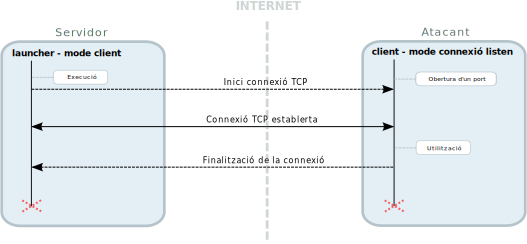
\includegraphics[scale=1,keepaspectratio]{diagrames/solutionDesignClientMode.pdf} \\
    \caption{Esquema del mode client}
    \label{fig:modeClient}
\end{figure}

Com veiem, en aquest mode el launcher i el client es canvien els papers, sent el launcher qui inicia una connexió 
cap al client. Aquest fet és el què li dona el nom al mode de funcionament. \\

Aquest mode de funcionament és molt interessant per el moment de la intrusió quan ja som capaços d'executar
comandes a la màquina. Evidentment per a poder fer ús d'aquest mode, cal que prèviament deixem el launxer 
a la màquina en qüestió. \\

Un cop fem això, el rootkit ens permetrà obtenir una shell enganxada a un TTY per tal de poder treballar 
còmodament, fer servir la màquina remota com a proxy SOCKS, així com pujar o baixar fitxers. Tenint en compte
que un cop acabi la connexió amb el rootkit, aquest haurà de tornar a ser llançat per a poder executar una següent
tasca. \\

\subsection{Mode servidor no privilegiat}

Aquest mode de funcionament no requereix de més privilegis que el mode client, però en aquest cas, si que
tindrem un servei executant-se a la màquina. \\

El fet de disposar d'un servei en constant execució o no, és la principal diferència entre el mode servidor
no privilegiat, i el mode client. En aquest mode, tindrem el launcher escoltant a un port TCP esperant que
el client es connecti per a sol·licitar una acció. \\

Aquest mode té l'inconvenient que en un entorn en què tinguem algun firewall, molt probablement, no ens 
servirà de res ja que les connexions cap al port del nostre launcher, molt probablement no estaran permeses. \\

\begin{figure}[htp]
    \centering
    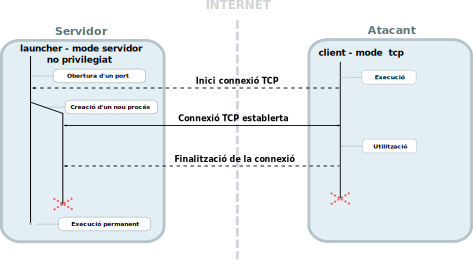
\includegraphics[scale=1,keepaspectratio]{diagrames/solutionDesignUnprivilegedServerMode.pdf} \\
    \caption{Esquema del mode servidor no privilegiat}
    \label{fig:modeUnprivilegedServer}
\end{figure}

\subsection{Mode servidor privilegiat}

El mode servidor privilegiat, és el mode que requereix de permisos d'administrador, i que alhora ens permetrà
fer ús de les característiques mes avançades del rootkit. \\

La principal diferència entre aquest mode de funcionament, és que al disposar de permisos d'administrador a
la màquina, podem realitzar tasques molt més avançades. Entre elles, tenim la possibilitat d'implementar 
sniffers a nivell d'aplicació per tal de poder capturar passwords, o el fet de poder utilitzar RAW sockets que
ens permetran utilitzar diferents modes de comunicació (se'n comenta el disseny més endavant), per tal de 
saltar-se la majoria de configuracions de firewall. \\

Per tots aquests motius, sempre que sigui possible ens interessarà utilitzar el rootkit en aquest mode. \\

El funcionament del rootkit quan s'està executant en mode privilegiat, varia depenent el tipus de connexió
que prefereix realitzar el client en aquell moment. Més endavant quan s'expliquen els modes de comunicació disponibles
en aquest mode (figures \ref{fig:modePrivilegedServerREV} i \ref{fig:modePrivilegedServerREV}), es detalla el seu funcionament. \\

\section{Modes de comunicació}

Tal i com hem comentat anteriorment, els modes de comunicació depenen directament dels permisos que tindrem 
a la màquina. Principalment per aquest motiu, s'han fet dependre dels modes de funcionament, és a dir, segons el
mode de funcionament, podrem utilitzar uns modes de comunicació o uns altres. \\

El rootkit implementa diferents modes de comunicació, alguns ens permeten establir connexions totalment
ocultes i arribar a sobrepassar configuracions de xarxa molt restrictives. Poder utilitzar un protocol de 
comunicació o un altre, dependrà del mode de funcionament en què hàgim arrancat el rootkit. És per aquest
motiu, que el mode de comunicació anirà molt lligat al mode de funcionament. \\

En total tenim quatre modes de comunicació. \\

\begin{enumerate}
    \item TCP
    \item REV
    \item RAW
    \item LISTEN
\end{enumerate}

La següent taula mostra quins modes de comunicació es poden utilitzar en cada mode de funcionament:

\begin{figure}[htp]
    \centering
    \begin{tabular}{|c|c|c|c|}
        \hline
               & \textbf{Client} & \textbf{Servidor no privilegiat} & \textbf{Servidor privilegiat} \\ \hline
        TCP    & \textcolor{Red}{No}   & \textcolor{Green}{Si} & \textcolor{Red}{No}  \\ \hline
        REV    & \textcolor{Red}{No}   & \textcolor{Red}{No}   & \textcolor{Green}{Si}  \\ \hline
        RAW    & \textcolor{Red}{No}   & \textcolor{Red}{No}   & \textcolor{Green}{Si}  \\ \hline
        LISTEN & \textcolor{Green}{Si} & \textcolor{Red}{No}   & \textcolor{Red}{No}    \\ \hline
    \end{tabular}
    \caption{Modes de comunicació disponibles segons el mode d'execució.}
    \label{fig:tableModesRelation}
\end{figure}

\subsection{TCP}

Aquest mode de comunicació, és utilitzat només en el cas en què el client vulgui connectar-se a un launcher que
s'ha executat en mode servidor no privilegiat. \\

El protocol de comunicació (figura \ref{fig:modeUnprivilegedServer}) en aquest cas és: \\

\begin{enumerate}
    \item El client estableix una connexió TCP amb a la màquina i port on està escoltant el launcher
    \item El client envia un paquet autenticat cap al launcher, especificant-li l'acció a portar a terme
    \item El launcher efectua l'acció, utilitzant la mateixa connexió ja establerta per a comunicar-se
\end{enumerate}

\subsection{REV}

Aquest mode de comunicació, es pot utilitzar només en el cas d'haver llançat el launcher en mode privilegiat.
El nom de REV, prové de la idea principal del mode de comunicació que és l'ús d'una comunicació reversa on 
és el client qui (a través d'un port ja obert en la màquina), sol·licita que el rootkit es connecti cap a ell. \\

El protocol de comunicació és el següent: \\

\begin{figure}[htp]
    \centering
    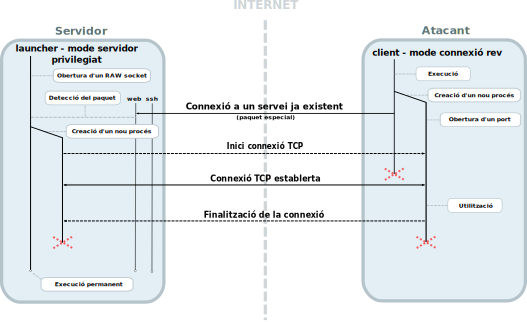
\includegraphics[scale=1,keepaspectratio]{diagrames/solutionDesignPrivilegedServerModeREV.pdf} \\
    \caption{Esquema del mode de connexió revers}
    \label{fig:modePrivilegedServerREV}
\end{figure}

\begin{enumerate}
    \item El client obre un servei que es queda escoltant a un port esperant la connexió del launcher.
    \item El client llança un procés fill que es connecta a un port TCP qualsevol de la màquina on s'està 
        executant el rootkit. Aquest port ha d'haver estat obert per qualsevol altre servei del sistema (per 
        exemple el típic servei web).
    \item El client envia un paquet autenticat través d'aquesta connexió. Aquest paquet serà probablement  
        descartat pel servei al no ser un paquet que compleixi el protocol del servei, però serà detectat per
        part del rootkit.
    \item El rootkit detectarà i comprovarà el paquet, i en cas de ser vàlid, establirà una connexió TCP cap 
        al client.
    \item Un cop establerta la connexió amb el client, s'utilitzarà aquesta per tal d'efectuar l'operació 
        demandada.
\end{enumerate}

Els principals avantatges son: \\

\begin{itemize}
    \item La comunicació entre launcher i client és molt fiable i és provable que sobrepassi la majoria de 
        configuracions de xarxa d'una manera totalment vàlida.
    \item Per executar el client, no necessitem permisos de superusuari.
\end{itemize}

Els principals desavantatges són: \\

\begin{itemize}
    \item El primer és que requerim que la màquina disposi d'alguna aplicació que escolti en algun port 
        TCP. Tot i que això no acostuma a ser difícil, hi han casos en què no és així.
    \item El segon és que un cop el rootkit ha establer la connexió TCP amb el client, aquesta connexió
        apareix en el llistat de connexions establertes de la màquina, i en segons quina màquina, això
        pot ser molt sospitós per a l'administrador.
\end{itemize}

Per tal d'utilitzar aquest mode de comunicació, cal que la màquina on s'executa el client, tingui almenys
un port de la ip pública, assignat a ella, de manera que sigui possible lo comunicació directe des de fora
la xarxa local. En configuracions personals com una línia ADSL amb router, caldria que el router de la màquina
on l'executés el client, tingués un ``port obert'' (un port amb DNAT) per tal que el rootkit es pogués 
connectar a ell. Aquest requisit també existeix en els següents modes de comunicació (RAW i LISTEN). \\

\subsection{RAW}

Igual que en el cas anterior, aquest mode de comunicació només pot ser utilitzat en cas d'haver llançat el launcher
en mode privilegiat. \\

Per tal d'implementar aquest mode de comunicació, s'ha hagut d'implementar un protocol de capa de transport 
compatible amb el subset de paquets vàlids pel protocol TCP (documentat més endavant). D'aquesta manera s'ha 
aconseguit poder transmetre per internet paquets TCP vàlids, que a nivell de sessió són aparentment invàlids. 
Com que tots aquests paquets són entregats a la màquina, el nostre rootkit és capaç d'interpretar-los i 
respondre obtenint com a resultat un protocol de comunicació invisible per el nucli del sistema operatiu. \\

Fer tot això, ens aporta principalment dos avantatges: \\

\begin{enumerate}
    \item Que les connexions establertes utilitzant aquest mode, són gairebé invisibles (caldria analitzar els
        diferents paquets de xarxa per detectar una connexió d'aquest tipus)
    \item Que no necessitem tenir cap aplicació escoltant a un port per tal de comunicar-nos amb el launcher.
\end{enumerate}

El nom de mode de comunicació RAW, prové del tipus de socket que ens permet implementar tot això (RAW socket),
i el seu funcionament és el següent: \\

\begin{figure}[htp]
    \centering
    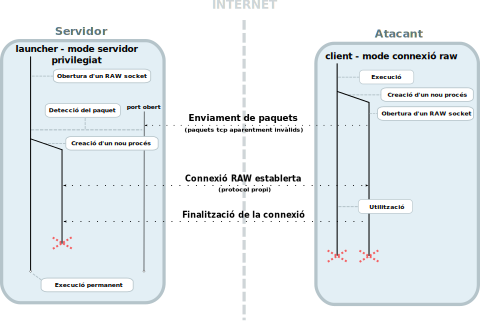
\includegraphics[scale=1,keepaspectratio]{diagrames/solutionDesignPrivilegedServerModeRAW.pdf} \\
    \caption{Esquema del mode de connexió revers}
    \label{fig:modePrivilegedServerRAW}
\end{figure}

\begin{enumerate}
    \item Primer de tot, el client inicialitza un socket RAW per tal de comunicar-se amb el launcher.
    \item El client crea un procés per tal d'enviar envia el paquet d'autenticació a la màquina i port escollits,
        i espera que el launcher li respongui.
    \item Un cop el launcher rep el paquet, comprova si el paquet és d'alguna connexió existent, i si no
        ho és, crea un altre procés destinat als enviaments de paquets cap al client. Alhora, comença a
        processar l'acció que li ha sol·licitat el client, tot utilitzant els paràmetres rebuts per a la 
        comunicació.
    \item En el moment que el client rep una resposta del launcher, comença a processar l'acció tenint
        ja la connexió establerta.
\end{enumerate}

\subsection{LISTEN}

Aquest mode de comunicació és el què s'utilitza amb el mode de funcionament client, i no requereix de permisos
especials per tal de ser utilitzat. En aquest cas, el client obre un servei per tal d'esperar la connexió del 
launcher.  \\

Es pot veure l'esquema en la figura \ref{fig:modeClient} \\

En el moment en què el client rep la connexió del launcher, aquest li sol·licita una acció en concret a executar
i passa a utilitzar la connexió establerta per a efectuar l'acció. \\

\section{Protocol de comunicació RAW}

L'objectiu de crear un protocol propi de comunicació, era aconseguir comunicar el client i el launcher per
internet sense que les utilitats del sistema operatiu per visualitzar les connexions de xarxa establertes
s'adonessin de les connexions entre launcher i client. En definitiva, l'objectiu és aconseguir passar més 
desapercebuts. \\

Per tal de poder aconseguir això i establir una comunicació a través d'internet, calia utilitzar un subset de 
paquets IP vàlids per a tota l'electrònica de xarxa que hi ha a internet. Per aquest motiu, es va escollir
utilitzar paquets vàlids del protocol TCP, però que són invàlids ja que fan referència a una sessió inexistent.
A més, per tal de afavorir que els paquets eren entregats, aquests eren enviats amb el flag de RESET activat. 
Aquesta peculiaritat fa que en alguns firewalls de baixa qualitat configurats amb una política de restricció de 
tots els paquets entrants menys els paquets que formen part d'una connexió ja establerta, detectin que el paquet
fa referència a una connexió ja establerta\footnote{Molts d'aquests firewalls, només afegeixen una regla denegant
els paquets amb el flag SYN, ja que només intenten denegar el inici d'una connexió TCP.} i el deixin passar. \\

Cal dir que aquest protocol es podria millorar força tot afegint algoritmes de control i retransmissió. Actualment
el nostre protocol de comunicació RAW, es podria dir que només ofereix les característiques del protocol UDP
\footnote{El protocol UDP és un protocol de transmissió que permet l'enviament de dades sense haver d'iniciar una 
sessió. Les dades enviades utilitzant aquest protocol, no són confirmades per el receptor i per tant la comprobació
s'ha de fer a nivell d'aplicació.}. Més endavant en el capítol solucions, s'explica amb tot detall el seu funcionament. \\

Els paquets transmesos per la xarxa segueixen aquesta estructura: \\

\begin{figure}[htp]
    \centering
    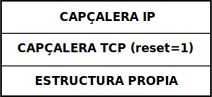
\includegraphics[scale=1,keepaspectratio]{diagrames/solutionDesignPacketStructure.pdf} \\
    \caption{Esquema d'un paquet RAW}
    \label{fig:packetScheme}
\end{figure}

En definitiva són paquets TCP amb el flag RESET activat, i una estructura de dades que detallem a continuació.

\subsection{Paquet de comunicació}

La següent estructura, s'utilitza en dos casos diferenciats:
\begin{itemize}
    \item L'enviament de paquets de control.
    \item L'enviament de paquets d'una connexió RAW.
\end{itemize}

Els paquets de control, són tots aquells que sol·liciten realitzar una acció tant del client al launcher, com a l'inrevés.
Els d'una connexió RAW són els comentats en el punt anterior.

El fet de que el client sol·liciti una acció al launcher, implica l'enviament d'un paquet de control del client sol·licitant
la realització d'una acció. 

\begin{Verbatim}[commandchars=@\[\]]
@PYay[struct] data {
    @PYaJ[unsigned] @PYaJ[char] pass@PYZlb[]@PYag[20]@PYZrb[];
    @PYaJ[unsigned] @PYaJ[char] action;
    @PYaJ[unsigned] @PYaJ[short] port;
    @PYaJ[unsigned] @PYaJ[long] size;
    @PYaJ[unsigned] @PYaJ[char] bytes@PYZlb[]BUFSIZE@PYZrb[];
} __attribute__ ((packed));
\end{Verbatim}

Podem veure que aquesta estructura conté un array de 20 bytes anomenat pass. És en aquest camp on tant el launcher
com el client s'han d'autenticar l'un amb l'altre, és a dir, tant el launcher ha de conèixer el password que ha introduït 
el client, com el client el client ha de conèixer el password amb el què va estar compilat el launcher.\\

Pel què fa als altres paràmetres, ``action'' fa referència a la acció\footnote{Es pot 
veure aquest camp, com el camp que especifica com ha de fer servir el valor dels altres pàmetres.}, ``port'' al port a 
utilitzar, ``size'' al nombre de bytes utiiltzats en el buffer ``bytes''.



% Sol.lució desenvolupada finalment
\section{Sol·lució}

        - Quan tenim el problema clar, cal pensar en una
        sol.lució, en aquest apartat de la memòria és on
        s'explica l'idea conceptual que solventa el
        problema presentat, tot es abstracte i no és té en
        compte cap limitació


% Estudi econòmic
\chapter{Estudi Econòmic}

En aquest capítol s'especifiquen les despeses de desenvolupament que s'han derivat de la realització
del rootkit portat a terme en aquest projecte. Aquestes despeses fan referència només al cost humà que
ha suposat, ja que pel què fa al material de treball utilitzat, s'ha utilitzat només material del què
ja disposàvem prèviament. \\

Per tal de quantificar el cost dels recursos humans, primer ens cal dividir els diferents participants
segons el rol que han portat a terme. En el nostre projecte, hi hem participat els següents rols.

\begin{itemize}
\item Doctor en Enginyeria Informàtica com a director del projecte.
\item Enginyer superior com a executor del projecte.
\end{itemize}

Per tal de poder quantificar el cost, ha estat necessari estimar un preu hora de
cadascun dels perfils. Així doncs, s'ha considerat que el preu hora de l'enginyer director és de 85\euro/h,
i el de l'enginyer executor del projecte és de 45\euro/h. Cal tenir en compte que l'enginyer executor és un
enginyer ja experimentat i amb força experiència en el món laboral. \\

\begin{figure}[htp]
\centering
\begin{tabular}{c c c c}
	\textbf{Perfil} & \textbf{Hores} & \textbf{Preu hora} & \textbf{Preu total} \\
	\hline
	Doctor en Enginyeria Informàtica & 100 & 85\euro & 8.500\euro \\
	Enginyer superior & 700 & 45\euro & 31.500\euro \\
	& & \textbf{Total} & 40.000\euro \\
\end{tabular}
\caption{Cost total del projecte}
\label{fig:costProjecte}
\end{figure}


% Conclussions
\chapter{Conclusions}
        - El capitol de conclussions, bàsicament fa una
        recapitulació de tots els objectius que s'havien
        marcat al capitol d'introducció/requeriments
        enumerant quins s'han aconseguit, i quins no,
        explicant el perquè, i les futures linies de treball.
Tenim un
        problema "volem comprometre sistemes UNIX", hem
        pensat una possible sol.lució (l'idea conceptual),
        tenim una idea més o menys clara del que cal fer i
        com fer-ho. Per tant, és viable fer-ho, però cal
        deixar-ho ben present a qui llegeixi la teva memòria.


% Apendix: 
\appendix

% Bibliografia
\clearpage
\phantomsection
\addcontentsline{toc}{chapter}{\numberline {10}Bibliografia}

\begin{thebibliography}{9}
 
\bibitem{dietlibc}
  Felix von Leitner,
  \emph{diet libc - a libc optimized for small size}.
  http://www.fefe.de/dietlibc/
  2009.
 
\end{thebibliography}


%http://en.wikipedia.org/wiki


% Glossari
\chapter{Glossari}
%\usepackage{syntonly}
%\syntaxonly
%\usepackage[style=list,toc=true]{glossary}
%\makeglossary
%\newacronym[PURL]{PURL}{persistent uniform resource locator}{description={A means of creating persistent links to 
%networked resources through the use of an intermediate resolution service.  The PURLs used in this thesis are 
%provided by the Online Computer Library Center (\url{http://purl.org}).}}
%\newacronym[PURL2]{GNU}{GNU s Not Unix}{description={A computer operating system composed entirely of free software.}}
%\newacronym{linux}{Linux}{description={Any Unix-like computer operating system that uses the Linux kernel.}}
%\newacronym{BSD}{Berkeley Software Distribution}{description={Sistema operatiu de la universitat de Berkeley. Sistema basat en UNIX.}}
%\newacronym{virus}{Virus}{description={Un virus informático es un malware que té per objectiu alterar el funcionament de la màquina.}}
%\newacronym{cavall de troia}{Cavall de troia}{description={}}
%\newacronym{malware}{Malware}{description={Peça de software que té un objectiu maliciós.}}
%\newacronym{rootkit}{Rootkit}{description={Èina o grup d'èines que té com a finalitat 
%amagar-se a ella mateixa, i amagar altres programaes, processos, arxius, directoris, ports, etc., 
%per tal que permeti a un intrús accedir al sistema principalment remotament, així com extreure informació.}}
%\makeindex


% Manual d'usuari
\chapter{Manual d'usuari}

A continuació s'han adjuntat els tres manuals en format ``man'' de UNIX dels dos executables que formen
el rootkit (skd-launcher i skd-client), i de les variables de configuració del launcher. 

\includepdf[pages=-]{skd-client.pdf}
\includepdf[pages=-]{skd-launcher.pdf}
\includepdf[pages=-]{skd-config.pdf}


\end{document}
